\chapter{2018:Constantinos Daskalakis}
\label{chap:daskalakis}
\begin{center}
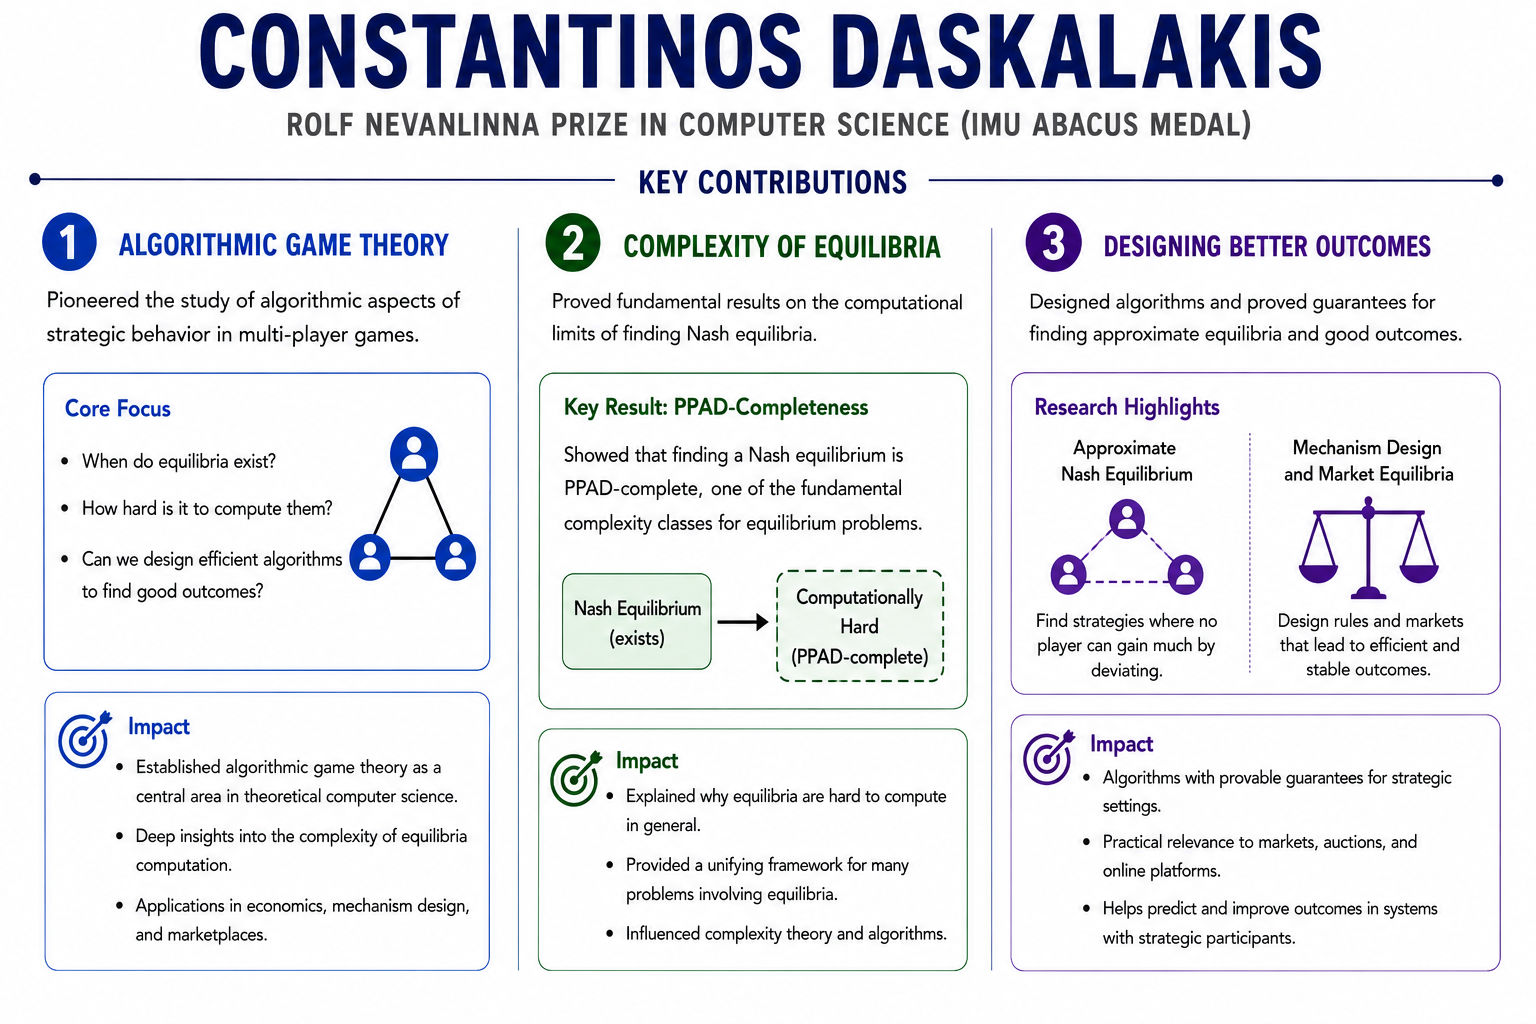
\includegraphics[width=\textwidth]{infographics/abacus10.png}
\end{center}
\targetchapterspacing
\index{Daskalakis, Constantinos}
\booknote{The central habit in this chapter is to keep existence and computation apart: a theorem that a solution exists is not an algorithm for finding it.}

\section{An Opening Story: A Price War Between Two Sellers}

Two coffee sellers, Priya and Malik, face each other across the same street. Each morning each posts a price for a latte, and each profit depends on the other's price: undercut by a dollar and the commuters drift to your window. So each seller's \emph{best} price is a moving target---whatever beats the other's price of yesterday. Starting from \$5 and \$5, Priya drops to \$4.50, Malik answers at \$5.25, Priya drops to \$4.25. They may settle on a stable pair, bounce forever, or wander.

A theorem guarantees a stable pair of prices exists: at some pair, neither seller, facing the other's price, would change anything. But the theorem does not say how to find it, nor what a month of daily adjustments will do. \emph{A stable pair exists} and \emph{here is how to find it} are different claims. This chapter is about the difference.

\section{The Problem}

In a game, each player's best choice depends on everyone else's. A \emph{Nash equilibrium} is a collection of choices---possibly random, since a player may prefer to mix---such that nobody can improve by changing alone. Nash proved in 1950 that every finite game has an equilibrium. That settled existence. The problem here is \emph{computation}: given the rules of a game, find an equilibrium. Existence and calculation are different questions, and a well-defined solution need not be algorithmically accessible.

\section{The World Before}

\noindent\textbf{Nash's proof was non-constructive.} Best responses form a set-valued correspondence rather than a continuous map, so the standard existence proof uses Kakutani's fixed-point theorem (or an equivalent continuous reformulation). The theorem guarantees an equilibrium in the compact convex region of mixed-strategy profiles but gives no recipe for locating it.

\noindent\textbf{Economists treated equilibria as predictions.} The equilibrium of a market---prices where supply meets demand---was a forecast, on the implicit assumption that players or markets would reach it. For decades nobody asked whether anyone or any algorithm could actually find one.

\noindent\textbf{Pivoting algorithms worked in practice.} The Lemke--Howson algorithm and its relatives find equilibria of two-player games by walking around the polytope of profiles. They solve small games quickly, but carry no general guarantee: some games force exponentially long walks.

\noindent\textbf{Continuous space, discrete search.} Brouwer's theorem lives in a continuous region; a computer searches a finite structure, and a grid does not help: a fixed point can sit between grid points, and the grid has exponentially many cells.

What was missing was a language for the difficulty of problems whose solutions are \emph{guaranteed} to exist. Classes like NP capture ``hard to decide''; for search problems with a promised answer, no comparable class existed, nor the reduction machinery to prove one such problem as hard as any other. Those tools were what Daskalakis and his collaborators supplied.

\section{The New Idea}
\subsection{The path picture: PPAD}

Consider a directed graph where every node has at most one arrow in and at most one arrow out. Such finite graphs split into paths and cycles. A node with no arrow entering is a \emph{source}; one with no arrow leaving is a \emph{sink}. Handed a source, following arrows must stop at a sink: the graph is finite, and a revisit would give some node a second incoming arrow---forbidden. The ends of paths come in pairs, and you were given one end.

Now make the graph \emph{implicit}: $2^k$ nodes, not listed, with a small circuit reporting each node's predecessor and successor. This is the setup of \textbf{PPAD} (Polynomial Parity Argument on Directed graphs): total search problems whose solution is guaranteed by exactly this parity/path argument. Given one endpoint of a path, find another---a node whose indegree differs from its outdegree. Following the path always works but may take $2^k$ steps.

\subsection{Nash equilibrium is PPAD-complete}

Daskalakis, Goldberg, and Papadimitriou showed that a game can encode the successor circuit of a PPAD problem: they built games with three or more players whose Nash equilibria encode the ``other end of the path'' of any PPAD instance, so finding an equilibrium is at least as hard as finding that endpoint. Chen and Deng extended this to two-player games; Chen, Deng, and Teng, even to \emph{approximate} equilibria when the allowed error is small. This was the first natural problem known to combine guaranteed existence with provable hardness of search. The difficulty is not a missing algorithm; it is a structural property of the problem class.

\subsection{The same framework, elsewhere}

The reduction template spread to market equilibria, auction bidding, and mechanism design: a solution exists by a fixed-point or parity argument, but computing it is hard in general. Not a blanket claim of hopelessness---special cases have fast algorithms: two-player zero-sum games solve by linear programming; potential games settle under any improving best responses; few players, limited interaction, or special payoffs admit dedicated algorithms. \emph{Easy structure versus hard general case is the whole point.}
\emph{The conceptual shift: a theorem that a solution exists is not an algorithm for finding it, and a problem can be guaranteed-solvable in principle yet provably intractable to search.}

\section{How It Works: Worked Examples}
\subsection{Matching pennies: finding the mixed equilibrium}

Row and Col each choose Heads ($H$) or Tails ($T$). Row receives $+1$ when the choices match and $-1$ when they differ; Col receives the opposite. This zero-sum game has no pure equilibrium: whichever pair you pick, one player wants to switch.

Let Row play $H$ with probability $p$. Against Col's $H$, Row's expected payoff is $p(+1)+(1-p)(-1)=2p-1$; against Col's $T$, it is $p(-1)+(1-p)(+1)=1-2p$. For Col to be willing to mix, Col must be indifferent between $H$ and $T$, so
\[
2p-1=1-2p \quad\Longrightarrow\quad 4p=2 \quad\Longrightarrow\quad p=\tfrac12,
\]
and by symmetry Col also plays $H$ with probability $\tfrac12$.

The equilibrium: both randomize 50/50, each with expected payoff $2p-1=0$. Check it: if Row switches to pure $H$ while Col randomizes, Row's expected payoff is $\tfrac12(+1)+\tfrac12(-1)=0$---no gain. Nobody can improve by deviating, which is the definition of equilibrium. Note the \emph{indifference principle}: at equilibrium, every action played with positive probability must give equal expected payoff, or the player would shift probability to the better one.

\subsection{The PPAD path: existence you can feel but not always walk}

Nodes $0,1,2,3,4$; edges $0\to1$, $1\to2$, $3\to4$. The graph is implicit: a successor circuit answers node by node,
\[
\operatorname{succ}(0)=1,\ \operatorname{succ}(1)=2,\ \operatorname{succ}(2)=\varnothing,\ \operatorname{succ}(3)=4,\ \operatorname{succ}(4)=\varnothing,
\]
with consistent predecessors $\operatorname{pred}(1)=0$, $\operatorname{pred}(2)=1$, $\operatorname{pred}(4)=3$. Sources (no incoming edge): $0$ and $3$; sinks (no outgoing edge): $2$ and $4$. Given source $0$, follow: $\operatorname{succ}(0)=1$, $\operatorname{succ}(1)=2$, $\operatorname{succ}(2)=\varnothing$. The walk stops at $2$: the other end. Two sources, two sinks---ends of paths come in pairs, so knowing one end guarantees another exists.

Why hard? Here the whole graph is drawn, so the answer is obvious. In a real instance the graph has $2^k$ nodes presented only through the circuits: you evaluate them one node at a time, never seeing the whole graph, and the path from your source can have length $2^k$. Walking it takes $2^k$ steps, though the guarantee that the other end exists is airtight. When the successor circuit encodes another hard problem, locating the other end is provably as hard as solving it.

\section{The Mathematics in Brief}

A \emph{finite game} has $n$ players with finite action sets $A_i$. A \emph{mixed strategy} for player $i$ is a distribution $x_i$ over $A_i$; a \emph{profile} $x=(x_1,\dots,x_n)$ collects one per player, giving expected payoff $u_i(x)$. Strategy $x_i$ is a \emph{best response} when $u_i(x_i,x_{-i})\ge u_i(y_i,x_{-i})$ for every $y_i$. A \emph{Nash equilibrium} is a profile where everyone plays a best response---a fixed point of the best-response correspondence. \emph{Why existence is true:} profiles form a compact convex region, each best-response set is nonempty and convex, and the correspondence is upper hemicontinuous; Kakutani's theorem supplies a fixed point.

The \emph{indifference principle} is the workhorse: at equilibrium, actions used with positive probability give equal expected payoff; worse actions get probability zero.

\textbf{PPAD} is the class of total search problems whose guaranteed solution follows from a path/parity argument on an implicitly defined graph: indegree and outdegree each $\le1$; given a source, find a node whose indegree differs from its outdegree. \emph{Why the guarantee holds:} following the unique path from a source cannot loop, so it must reach a sink.

\textbf{The completeness theorem.} Computing a Nash equilibrium of a game with three or more players is PPAD-complete (Daskalakis--Goldberg--Papadimitriou), and remains so for two-player games and even for \emph{approximate} equilibria (Chen--Deng; Chen--Deng--Teng). An $\varepsilon$-equilibrium is a profile where $u_i(x_i,x_{-i})+\varepsilon\ge u_i(y_i,x_{-i})$ for all $y_i$: nobody gains more than $\varepsilon$ by deviating. \emph{Why:} games can encode successor circuits, so an equilibrium encodes the endpoint of a hidden path. \emph{Consequence:} worst-case hardness coexists with fast algorithms on structured instances, and with learning dynamics that may converge to outcomes that are not equilibria.

\section{Limits and Modern Views}

PPAD-completeness is a \emph{worst-case} statement, asymptotic in game size. It does not say real markets are unsolvable: practical instances usually carry structure---few players, symmetric payoffs, sparse interaction---that dedicated algorithms exploit.

Approximation does not dissolve the difficulty: an $\varepsilon$-equilibrium is hard when the required precision is part of the input, and the smaller the error, the more of the hard problem the game encodes. Discretization is no escape: replacing a continuous strategy space by a finite grid changes the game, and the discrete equilibria need not lie near the continuous ones. Learning dynamics may cycle or settle into stable non-equilibrium outcomes---for prediction, those may matter more than the equilibrium itself, shifting the question from \emph{what is the equilibrium?} to \emph{what outcomes can plausible processes generate?}

The field that grew from these results is \emph{algorithmic economics}: auctions and mechanisms where truthfulness, feasibility, and computation fit together. Optimal transport supplies a geometric language for some mechanism-design problems, dual potentials playing the role of prices. The deep lesson: social concepts have computational structure---equilibrium, incentive compatibility, and optimal allocation are algorithmic tasks whose representations determine what can be found, approximated, or predicted \cite{daskalakis-nash,daskalakis-markets}.

\section{Exercises and Self-Study Guide}
\begin{enumerate}[label=\textbf{E\arabic*.}]
\item Biased matching pennies: Row gains $+3$ when both play $H$, $+1$ when both play $T$, $-1$ on a mismatch; Col's payoffs are the negatives. If Row plays $H$ with probability $p$ and Col with probability $q$, find the equilibrium $(p,q)$ and Row's expected payoff.
\hint{Col's mix $q$ must make Row indifferent: equate $q(+3)+(1-q)(-1)$ with $q(-1)+(1-q)(+1)$; then use $p$ to make Col indifferent.}
\item In ordinary matching pennies, show (both play $H$) is an $\varepsilon$-equilibrium for $\varepsilon=2$ but not an equilibrium, and that no pure profile is an equilibrium.
\hint{At $(H,H)$ Row gets $+1$, Col $-1$; compute the best each could do by switching alone and take the larger gain.}
\item Explain why Nash's fixed-point existence proof gives no search algorithm.
\hint{Brouwer guarantees a point but no path to it; a grid search either misses it or faces exponentially many cells.}
\item Trace best-response dynamics in matching pennies from $(H,H)$ and show the play cycles forever.
\hint{Row copies Col and Col plays the opposite: $(H,H)\to(H,T)\to(T,T)\to(T,H)\to(H,H)$.}
\item A seller's price is continuous in $[4,7]$ with unique equilibrium $\$5.37$. Explain how forcing prices onto the grid $\{4,5,6,7\}$ can change the equilibrium.
\hint{The grid game allows different deviations and output points; the continuous equilibrium may lie strictly between grid lines.}
\item No-regret learners in matching pennies never settle, yet their empirical frequencies converge to the equilibrium mix. Why is stable frequency compatible with unstable play?
\hint{Regret compares accumulated average payoff with the best fixed action; in a zero-sum game the frequencies encode the equilibrium while realized actions alternate.}
\item Pick one assumption a market or mechanism-design model relies on---quasi-linear utilities, a known type distribution, or fully rational agents---and explain what happens to the complexity analysis if it is removed.
\hint{Ask which part of the argument used it: a truthfulness proof needs quasi-linear utility, a hardness reduction needs structure encoding arbitrary instances---removing it reopens the complexity question.}
\end{enumerate}

\booknote{A final exercise in judgment: whenever you are told that a solution exists, ask separately how a machine would find it, how the answer would be verified with a certificate, and whether the guarantee survives approximation. If you cannot name the certificate, the existence proof is not yet an algorithm.}
\clearpage
